\documentclass[a4paper,12pt]{article}
\usepackage[utf8]{inputenc}
\usepackage[russian]{babel}
\usepackage{amsmath, amssymb}
\usepackage{graphicx}
\usepackage{geometry}
\geometry{top=2cm, bottom=2cm, left=2.5cm, right=2cm}
\usepackage{float}

\begin{document}
	
	\begin{center}
		\Large\textbf{Численное решение краевой задачи для уравнения Пуассона} \\
	\end{center}
	
	\section*{Постановка задачи}
	
	Рассматривается одномерная краевая задача для уравнения Пуассона:
	\begin{equation}
		-u''(x) = f(x), \quad x \in (0, L)
		\label{eq:poisson}
	\end{equation}
	с граничными условиями:
	\begin{equation}
		u(0) = u_0, \quad u(L) = u_L
		\label{eq:bc}
	\end{equation}
	
	Требуется найти приближенное решение задачи (\ref{eq:poisson})-(\ref{eq:bc}) методом конечных разностей и исследовать сходимость численного решения к точному.
	
	\section*{Точное решение}
	
	В качестве тестовой задачи выбрано уравнение с правой частью:
	\begin{equation}
		f(x) = -25\sin(4x)\cos(3x) - 24\cos(4x)\sin(3x)
		\label{eq:f}
	\end{equation}
	Точное решение имеет вид:
	\begin{equation}
		u_{\text{exact}}(x) = \sin(4x)\cos(3x)
		\label{eq:exact}
	\end{equation}
	
	Граничные условия:
	\begin{equation}
		u(0) = 0, \quad u(L) = \sin(4L)\cos(3L), \quad L = 1
	\end{equation}
	
	\section*{Численный метод}
	
	\subsection*{Дискретизация}
	
	Введем равномерную сетку на отрезке $[0, L]$:
	\begin{equation}
		x_i = i h, \quad i = 0, 1, \dots, n+1, \quad h = \frac{L}{n+1}
	\end{equation}
	где $n$ — количество внутренних узлов.
	
	\subsection*{Разностная схема}
	
	Вторую производную аппроксимируем центральной разностью:
	\begin{equation}
		-u''(x_i) \approx -\frac{u_{i-1} - 2u_i + u_{i+1}}{h^2} = f(x_i)
	\end{equation}
	
	После умножения на $-h^2$ получаем систему линейных уравнений:
	\begin{equation}
		-u_{i-1} + 2u_i - u_{i+1} = h^2 f(x_i), \quad i = 1, \dots, n
	\end{equation}
	
	\subsection*{Учет граничных условий}
	
	Для первого и последнего уравнений граничные условия учитываются переносом известных значений в правую часть:
	\begin{align}
		2u_1 - u_2 &= h^2 f(x_1) + u_0 \\
		-u_{n-1} + 2u_n &= h^2 f(x_n) + u_{n+1}
	\end{align}
	
	\subsection*{Метод прогонки}
	
	Полученная система имеет трехдиагональную матрицу и решается методом прогонки (алгоритм Томаса) за $O(n)$ операций. Прямой ход исключает нижнюю диагональ, обратный ход вычисляет значения неизвестных.
	
	\section*{Результаты вычислений}
	
	Для исследования сходимости были проведены расчеты при различных значениях $n$ от 5 до 1000 с шагом 5. Для каждого $n$ вычислялись следующие нормы ошибки:
	
	\begin{itemize}
		\item Чебышёвская (максимальная) норма:
		\begin{equation}
			\|e\|_{\infty} = \max_{1 \leq i \leq n} |u_{\text{num}}(x_i) - u_{\text{exact}}(x_i)|
		\end{equation}
		
		\item $L_2$ норма:
		\begin{equation}
			\|e\|_2 = \sqrt{h \sum_{i=1}^{n} |u_{\text{num}}(x_i) - u_{\text{exact}}(x_i)|^2}
		\end{equation}
	\end{itemize}
	
	\subsection*{График сходимости}
	
	\begin{figure}[H]
		\centering
		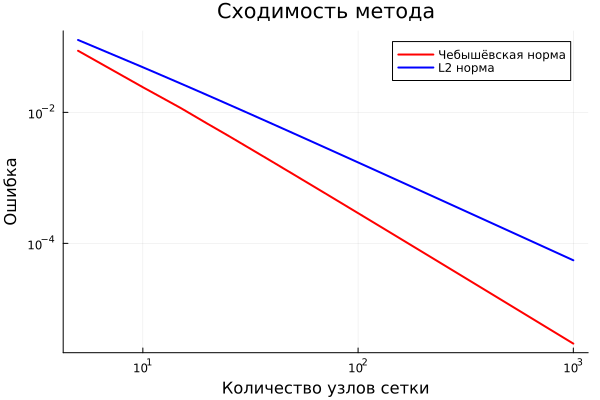
\includegraphics[width=0.8\textwidth]{result.png}
		\caption{Сходимость численного решения при увеличении числа узлов сетки}
		\label{fig:convergence}
	\end{figure}
	
\end{document}